%% by Michael Shell
%% Edited by Rodrigo Almeida
%%
%% This work is distributed under the LaTeX Project Public License (LPPL)
%% ( http://www.latex-project.org/ ) version 1.3, and may be freely used,
%% distributed and modified. A copy of the LPPL, version 1.3, is included
%% in the base LaTeX documentation of all distributions of LaTeX released
%% 2003/12/01 or later.
%% Retain all contribution notices and credits.

\documentclass[10pt,journal,compsoc]{IEEEtran}

\hyphenation{op-tical net-works semi-conduc-tor}


\usepackage{hyperref}
\usepackage{biblatex}
\usepackage{graphicx}
\usepackage{listings}
\usepackage{multirow}
\usepackage{tabularx}
\usepackage{caption}
\usepackage{booktabs}

\graphicspath{{images/}}

\addbibresource{references.bib}

\begin{document}
% paper title
% Titles are generally capitalized except for words such as a, an, and, as,
% at, but, by, for, in, nor, of, on, or, the, to and up, which are usually
% not capitalized unless they are the first or last word of the title.
% Linebreaks \\ can be used within to get better formatting as desired.
% Do not put math or special symbols in the title.

\title{Gesture UI Project Report}

% author name
\author{Rodrigo Almeida - G00377123% <-this % stops a space
}

% The paper headers
\markboth{Atlantic Technological University - Gesture UI}%
{}

% make the title area
\maketitle

\section{Introduction}
\label{sec:introduction}

\IEEEPARstart{T}his project undertakes a comprehensive analysis of the dataset \textit{Traffic, Driving Style and Road Surface Condition} \cite{dataset}. The dataset includes low-level parameters
gathered through On-Board Diagnosis II (OBD-II) interfaces in vehicles and accelerometers embedded in smartphones. The data collection approach aimed to capture the dynamics between the driver's vehicles, and
environmental conditions. The dataset focuses on data related to two specific car models - Peugeot 207 1.4 HDi and Opel Corsa 1.3 HDi.
The project aims to compare the efficacy of three classification algorithms - Support Vector Machine (SVM), Logistic Regression, and K-Nearest Neighbors, through deep data preprocessing, 
feature engineering, and application of cross-validation techniques, seeking to optimize model performance.


\section{Methodology}

\subsection{Data Pre-processing}

One of the biggest challenges in machine learning is the quality of the data. The quality of 
the data is crucial to the performance of the model. The raw dataset comes from Kaggle \cite{dataset} 
and comprises data gathered from two diesel cars and are presumed to be two distinct road types, resulting in the dataset being partitioned across four CSV files. 
Each vehicle's data is represented in two separate files, each corresponding to a different road condition encountered during the data collection phase. The collected dataset was then labelled for three key attributes: 
\textit{traffic conditions, driving style, and road surface quality}, which makes it well suited for supervised learning. With the attributes specifically labelled, it is a classification issue. 

The data pre-processing phase is a critical step in the machine learning pipeline. It involves cleaning, transforming, and preparing the data for the model. 

\subsubsection{Imbalanced Dataset}
On the dataset, the number of instances for each class was found to be imbalanced, which can lead to poor performance of the model. 

Below is a description and number of instances for each class in the dataset:

\begin{itemize}
    \item \textbf{Driving Style:}
    \begin{itemize}
        \item EvenPaceStyle: 21,016 instances
        \item AggressiveStyle: 2,759 instances
    \end{itemize}
    \item \textbf{Road Surface Condition:}
    \begin{itemize}
        \item SmoothCondition: 14,237 instances
        \item UnevenCondition: 6,289 instances
        \item FullOfHolesCondition: 3,249 instances
    \end{itemize}
    \item \textbf{Traffic Condition:}
    \begin{itemize}
        \item LowCongestionCondition: 17,764 instances
        \item HighCongestionCondition: 3,017 instances
        \item NormalCongestionCondition: 2,994 instances
    \end{itemize}
\end{itemize}

For this project, \textit{Driving Style} class column was chosen due to its significant imbalance and potential for improvement. 
The \textit{AggressiveStyle} class has 2,759 instances while the \textit{EvenPaceStyle} class has 21,016 instances. The dataset is imbalanced, 
and the model may be biased towards the majority class. To resolve the issue of the imbalanced dataset that was observed, the use of other techniques such as over-sampling and under-sampling was considered.
SMOTE (Synthetic Minority Over-sampling) which is a statistical technique for increasing the number of instances in the minority class was used. SMOTE works by selecting
examples that are close to the feature space, drawing a line between the examples in the feature space and drawing a new sample at a point along that line. 
It does have some limitations, such as the generation of noisy samples, but it is a widely used technique for dealing with imbalanced datasets. \cite{fernandez2018smote}. 
Below is what the \textit{Driving Style} dataset looks like after applying SMOTE.

\begin{itemize}
    \item \textbf{Driving Style:}
    \begin{itemize}
        \item EvenPaceStyle: 16,808 instances
        \item AggressiveStyle: 16,808 instances
    \end{itemize}
\end{itemize}

With the dataset now balanced, the next step was to remove the \textbf{Unnamed: 0} column. This column was not needed for the analysis and was removed from the dataset.
After having that completed it was found that there were missing values in the dataset as shown in Table \ref{table:data_missing_values}.

\begin{table}[h]
    \centering    
    \begin{tabular}{|l|l|}
    \hline
    \textbf{Column}                   & \textbf{Missing Values} \\ \hline
    VehicleSpeedInstantaneous         & 9                       \\ \hline
    EngineLoad                        & 5                       \\ \hline
    EngineCoolantTemperature          & 5                       \\ \hline
    ManifoldAbsolutePressure          & 5                       \\ \hline
    EngineRPM                         & 5                       \\ \hline
    MassAirFlow                       & 5                       \\ \hline
    IntakeAirTemperature              & 5                       \\ \hline
    FuelConsumptionAverage            & 5                       \\ \hline
    \end{tabular}
    \caption{Missing Values in the Dataset}
    \label{table:data_missing_values}
\end{table}

Due to the small number of missing values relative to the size of the dataset, imputation seems to be a practical approach. For the numerical columns with missing values, it can be filled
with the mean or median of the column. For the categorical columns, the missing values can be filled with the mean of the column.
In this case was chosen to fill the missing values with the mean of the column, as it data is normally distributed.

\subsection{Data Labelling}

For the categorical variables - \textit{roadSurface}, \textit{traffic}, \textit{drivingStyle} - it was converted into a format that can be used for machine learning models. 
Since \textit{drivingStyle} is the target variable it was encoded using the \textit{LabelEncoder} from the \textit{sklearn.preprocessing} module and is now represented as 0 and 1. The continuous feature, on columns such as \textit{AltitudeVariation}, 
\textit{VehicleSpeedInstantaneous}, \textit{VehicleSpeedVariation}, are now standardized and centered around 0(mean) and 1(standard deviation). 
The categorical variables \textit{roadSurface} and \textit{traffic} are encoded using the \textit{OneHotEncoder} from the \textit{sklearn.preprocessing} module. Each column represents
the presence (True/1) or absence (False/0) of a category.

\subsection{Data Scaling}

Feature scaling is a method used to standardize the range of independent variables or features of the data. In data processing, it is also known as data 
normalization and is generally performed during the data pre-processing step.

The \textit{Standard Scaler} was used to scale the data. The Standard Scaler standardizes the features by removing the mean and scaling to unit variance.
This results in a distribution with a standard deviation of 1 and a mean of 0. The formula for standard scaling is given by:

\begin{equation}
    z = \frac{x - \mu}{\sigma}
\end{equation}

Where $x$ is the original feature value, $\mu$ is the mean of the feature, and $\sigma$ is the standard deviation of the feature. This process of subtracting the mean and 
dividing by the standard deviation ensures that all features contribute equally to the result, a critical consideration for algorithms like Support Vector Machines (SVM), 
k-Nearest Neighbors (kNN), and Logistic Regression were used in this project.


\subsection{Data Analysis and Visualisation}

As part of the analysis aiming to classify the driving styles, the data was visualized to understand the distribution of the features and the relationship between the features 
and the target variable. The PCA (Principal Component Analysis) was used to visualize the data in 2D. The PCA is a dimensionality reduction technique that is used to reduce the
dimensionality of the data to 2 or 3 dimensions so that it can be visualized. \cite{niedoba2014multi}

\begin{figure}
    \centering
    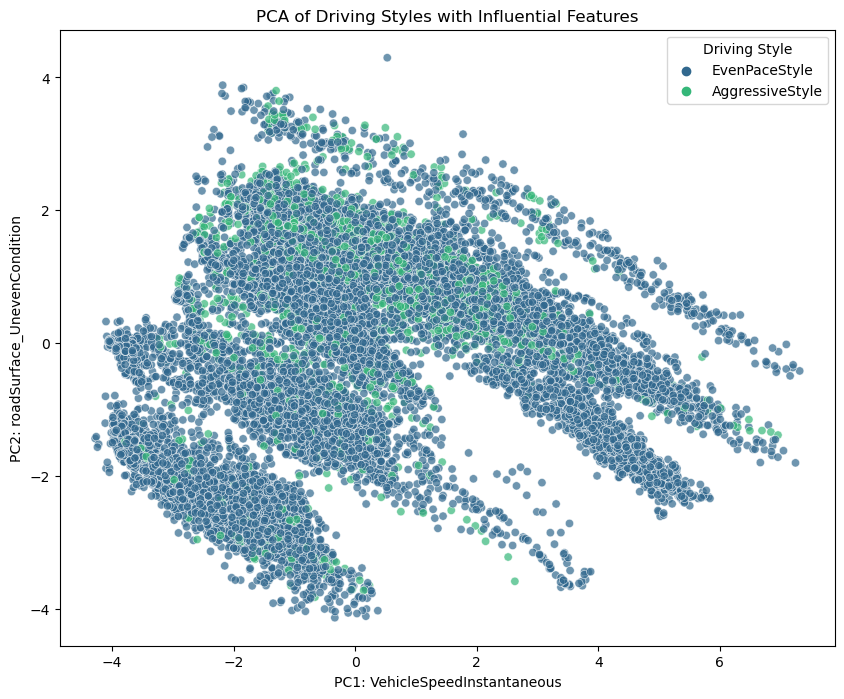
\includegraphics[width=0.5\textwidth]{images/pca_chart.png}
    \caption{PCA Visualization of the Data}
    \label{fig:pca}
\end{figure}

Figure \ref{fig:pca} shows the PCA visualization of the data. The classes are not well separated, suggesting the data is not
linearly separable and a linear model may not be the best choice for this dataset.
The axes are labelled as PC1: \textit{VehicleSpeedInstantaneous} and PC2: \textit{RoadSurface\_UnevenCondition}, implying that these two features contribute most to the variance in the data.
\textit{VehicleSpeedInstantaneous} might be a defining characteristic of the driving style, while \textit{RoadSurface\_UnevenCondition} might also influence the driving style.
Despite some level of separation, there is also significant overlap between the classes, which indicates that not all driving style characteristics are captured by these two features, or that there
maybe a wide range of behaviours within each style that could cause this overlap.
The presence of clusters in the data suggests a potential for classification models to predict the driving style based on the features.


\section{Experiments and Results}
\subsection{Linear Regression Model}
Now, with the knowledge about the imbalanced dataset, the new dataset processed with SMOTE was used to train the linear regression model. To find the best parameters for the model,
the \textit{GridSearchCV} method was used to find the best parameters for the model. The results from \textit{GridSearchCV} indicated that the best parameter for $C$ was \textit{0.1},
which was used to train the model. The model was then evaluated, using the balanced dataset and the results are shown in Table \ref{table:log_classification_report} 
and Table \ref{table:log_confusion_matrix}. The F1-Score of \textit{0.36} indicates that the model was able to identify \textit{AggressiveStyle} to some extent, but it is not very precise. On the other hand an F1-Score of \textit{0.80} 
for \textit{EvenPaceStyle} indicates that despite some misclassifications, the models generally perform well for this class. The overall accuracy of the model was \textit{70\%}.


\begin{table}[h]
    \centering    
    \begin{tabular}{|l|l|l|l|l|}
    \hline
    \textbf{Class} & \textbf{Precision} & \textbf{Recall} & \textbf{F1-score} & \textbf{Support} \\ \hline
    AggressiveStyle & 0.24 & 0.73 & 0.36 & 547 \\ \hline
    EvenPaceStyle & 0.95 & 0.69 & 0.80 & 4208 \\ \hline
    \textbf{Accuracy} & \multicolumn{4}{c|}{0.70} \\ \hline
    \textbf{Macro Avg} & 0.59 & 0.71 & 0.58 & 4755 \\ \hline
    \textbf{Weighted Avg} & 0.87 & 0.70 & 0.75 & 4755 \\ \hline
    \end{tabular}
    \caption{Classification Report for Logistic Regression}
    \label{table:log_classification_report}
\end{table}

% Confusion Matrix for Logistic Regression
\begin{table}[h]
    \centering
    \begin{tabular}{|c|c|c|}
    \hline
    \multicolumn{3}{|c|}{\textbf{Confusion Matrix for Logistic Regression}} \\
    \hline
    \textbf{Actual/Predicted} & \textbf{AggressiveStyle} & \textbf{EvenPaceStyle} \\ \hline
    \textbf{AggressiveStyle} & 398 & 149 \\ \hline
    \textbf{EvenPaceStyle} & 1284 & 2924 \\ \hline
    \end{tabular}
    \caption{Confusion Matrix for Logistic Regression}
    \label{table:log_confusion_matrix}
\end{table}

After optimizing the model parameters and evaluating its predictive performance, it is important to understand which features contribute most significantly to the model's predictions. 
In logistic regression, the coefficients associated with each feature can indicate the importance and influence of that feature on the model's output. 

To visualize the impact of each feature, a coefficient plot was constructed. This plot ranks the features by their coefficients, providing clear insights into which features are 
most informative for predicting the target variable.

\begin{figure}[h]
    \centering
    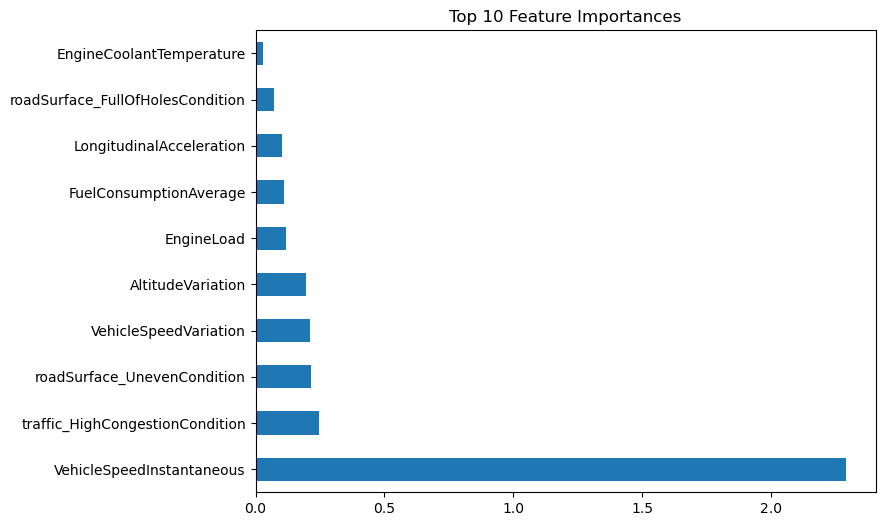
\includegraphics[width=0.5\textwidth]{images/feature_importance.png} 
    \caption{Top 10 Feature Importance in the Logistic Regression Model}
    \label{fig:feature_importances}
\end{figure}

This coefficient plot shows the relative importance of features in predicting driving styles. Features with larger absolute values of coefficients have a greater impact on the model's 
decision-making process. It is a good way to understand which features are most important for the model's predictions. The top 10 features are shown in Figure ~\ref{fig:feature_importances}.


\subsection{Support Vector Machine Model}
Before training the model with the Support Vector Machine (SVM), a range of $C$ values and Kernels - linear, poly, rbf and sigmoid were tested to find the optimal value. The model 
was trained using the \textit{GridSearchCV} method from the \textit{sklearn.model\_selection} module. The best $C$ and best $Kernel$ parameters were identified through cross-validation, optimizing for model accuracy. 
The best parameters and corresponding score obtained from the grid search were accessed via \texttt{svm\_grid.best\_params\_} and \texttt{svm\_grid.best\_score\_}, respectively. For this model, the best parameters were $C=10$, 
suggesting that the model has settled on a middle ground and $Kernel=rbf$ as it can handle non-linear data.

Before proceeding to evaluate the model with the balanced and pre-processed dataset, the model was trained using the original dataset to see how it would perform. The accuracy of the model
was evaluated returning a score of \textit{0.88}. But then, when running the classification report, it was found that the model was biased towards the majority class as shown in 
Table \ref{table:svm_classification_report}.
It is shown that the model was able to predict the majority class with a precision of \textit{0.88} and a recall of \textit{1.00}, but the minority class was not predicted at all. This is a clear indication of the model bias towards 
the majority class, this is due to the imbalanced nature of the dataset.

\begin{table}[h]
    \centering
    \begin{tabular}{|l|l|l|l|l|}
    \hline
    \textbf{Class} & \textbf{Precision} & \textbf{Recall} & \textbf{F1-score} & \textbf{Support} \\ \hline
    AggressiveStyle & 0.00 & 0.00 & 0.00 & 547 \\ \hline
    EvenPaceStyle & 0.88 & 1.00 & 0.94 & 4208 \\ \hline
    \textbf{Accuracy} & \multicolumn{4}{c|}{0.88} \\ \hline
    \textbf{Macro Avg} & 0.44 & 0.50 & 0.47 & 4755 \\ \hline
    \textbf{Weighted Avg} & 0.78 & 0.88 & 0.83 & 4755 \\ \hline
    \end{tabular}
    \caption{SVM Classification Report with imbalanced dataset}
    \label{table:svm_classification_report}
\end{table}

\begin{table}[h]
    \centering
    \begin{tabular}{|c|c|c|}
    \hline
    \multicolumn{3}{|c|}{\textbf{Confusion Matrix}} \\
    \hline
    \textbf{Actual/Predicted} & \textbf{AggressiveStyle} & \textbf{EvenPaceStyle} \\ \hline
    \textbf{AggressiveStyle} & 0 & 547 \\ \hline
    \textbf{EvenPaceStyle} & 0 & 4208 \\ \hline
    \end{tabular}
    \caption{SVM Confusion Matrix with imbalanced dataset}
    \label{table:confusion_matrix}
\end{table}

After applying SMOTE to the dataset, Table \ref{table:classification_report_smote} shows improvement in the model's ability to predict the minority class, which was not predicted at all 
in the previous trial. There seems to be a trade-off; as recall increased, precision decreased. This is expected as the model is now predicting more instances of the minority class.
A precision of \textit{0.43} for \textit{AggressiveStyle} and a high precision of \textit{0.98} for \textit{EvenPaceStyle} show a significant improvement compared to the Logistic Regression Model.
The recall of \textit{0.84} and \textit{0.86} respectively, demonstrate the model's sensitivity to picking up on the driving behaviours but also indicate that the model misses about \textit{15\%} of actual driving instances. 
The F1-score of\textit{0.57} for \textit{AggressiveStyle} show a balance between precision and recall, considering both false positives and false negatives for this class. The F1-Score of \textit{0.91} for \textit{EvenPaceStyle} is 
very good and indicates the model's performance in classifying the majority class. The overall accuracy of the model was \textit{0.85} meaning it correctly classifies \textit{85\%} of all instances, showing a greate 

\begin{table}[h]
    \centering    
    \begin{tabular}{|l|l|l|l|l|}
    \hline
    \textbf{Class} & \textbf{Precision} & \textbf{Recall} & \textbf{F1-score} & \textbf{Support} \\ \hline
    AggressiveStyle & 0.43 & 0.84 & 0.57 & 547 \\ \hline
    EvenPaceStyle & 0.98 & 0.86 & 0.91 & 4208 \\ \hline
    \textbf{Accuracy} & \multicolumn{4}{c|}{0.85} \\ \hline
    \textbf{Macro Avg} & 0.70 & 0.85 & 0.74 & 4755 \\ \hline
    \textbf{Weighted Avg} & 0.91 & 0.85 & 0.87 & 4755 \\ \hline
    \end{tabular}
    \caption{SVM Classification Report with dataset processed with SMOTE}
    \label{table:classification_report_smote}
\end{table}

% Confusion Matrix
\begin{table}[h]
    \centering
    \begin{tabular}{|c|c|c|}
    \hline
    \multicolumn{3}{|c|}{\textbf{Confusion Matrix}} \\
    \hline
    \textbf{Actual/Predicted} & \textbf{AggressiveStyle} & \textbf{EvenPaceStyle} \\ \hline
    \textbf{AggressiveStyle} & 458 & 89 \\ \hline
    \textbf{EvenPaceStyle} & 606 & 3602 \\ \hline
    \end{tabular}
    \caption{SVM Confusion Matrix with dataset processed with SMOTE}
    \label{table:confusion_matrix_smote}
\end{table}


\subsection{K-Nearest Neighbors Model}
The k-Nearest Neighbors (kNN) model was trained using the balanced dataset and the results are shown in Table \ref{table:knn_classification_report} and Table \ref{table:knn_confusion_matrix}.
With a precision of \textit{0.59}, the kNN model correctly predicts \textit{AggressiveStyle} \textit{59\%} of the time, this is an improvement compared to both the SVM and Logistic Regression models, 
suggesting fewer false positives for \textit{AggressiveStyle}. The precision for \textit{EvenPaceStyle} is very high at \textit{0.98} similar to SVM, indicating that the model is highly accurate when predicting even-paced driving.
The F1-Score of \textit{0.69} for \textit{AggressiveStyle} show a balance between precision and recall with a significant improvement over both SVM and Logistic Regression models. The F1-Score for \textit{EvenPaceStyle} 
was \textit{0.95}, which is very strong showing a good performance when classifying the majority class. The overall accuracy of \textit{0.91} shows that the kNN model correctly classifies \textit{91\%} of all instances, which is 
the highest accuracy among the three models.

\begin{table}[h]
    \centering    
    \begin{tabular}{|l|l|l|l|l|}
    \hline
    \textbf{Class} & \textbf{Precision} & \textbf{Recall} & \textbf{F1-score} & \textbf{Support} \\ \hline
    AggressiveStyle & 0.59 & 0.84 & 0.69 & 547 \\ \hline
    EvenPaceStyle & 0.98 & 0.92 & 0.95 & 4208 \\ \hline
    \textbf{Accuracy} & \multicolumn{4}{c|}{0.91} \\ \hline
    \textbf{Macro Avg} & 0.78 & 0.88 & 0.82 & 4755 \\ \hline
    \textbf{Weighted Avg} & 0.93 & 0.91 & 0.92 & 4755 \\ \hline
    \end{tabular}
    \caption{Classification Report for k-Nearest Neighbors (kNN)}
    \label{table:knn_classification_report}
\end{table}


\begin{table}[h]
    \centering
    \begin{tabular}{|c|c|c|}
    \hline
    \multicolumn{3}{|c|}{\textbf{Confusion Matrix for k-Nearest Neighbors (kNN)}} \\
    \hline
    \textbf{Actual/Predicted} & \textbf{AggressiveStyle} & \textbf{EvenPaceStyle} \\ \hline
    \textbf{AggressiveStyle} & 458 & 89 \\ \hline
    \textbf{EvenPaceStyle} & 320 & 3888 \\ \hline
    \end{tabular}
    \caption{Confusion Matrix for k-Nearest Neighbors (kNN)}
    \label{table:knn_confusion_matrix}
\end{table}

\subsection{Results}
The kNN generally showed the best performance across most metrics, especially in terms of balanced precision and recall for both classes. SVM came after, 
showing its strength in recall for \textit{AggressiveStyle}. Logist regression, while less precise for \textit{AgressiveStyle}, still provided insights due 
to the model's simplicity and interpretability. All models had to deal with class imbalances present in the data, which influenced their ability to predict the less represented 
\textit{AgressiveStyle} accurately. The SMOTE technique helped address this issue, improving all model's performance. 

\begin{figure}[h]
    \centering
    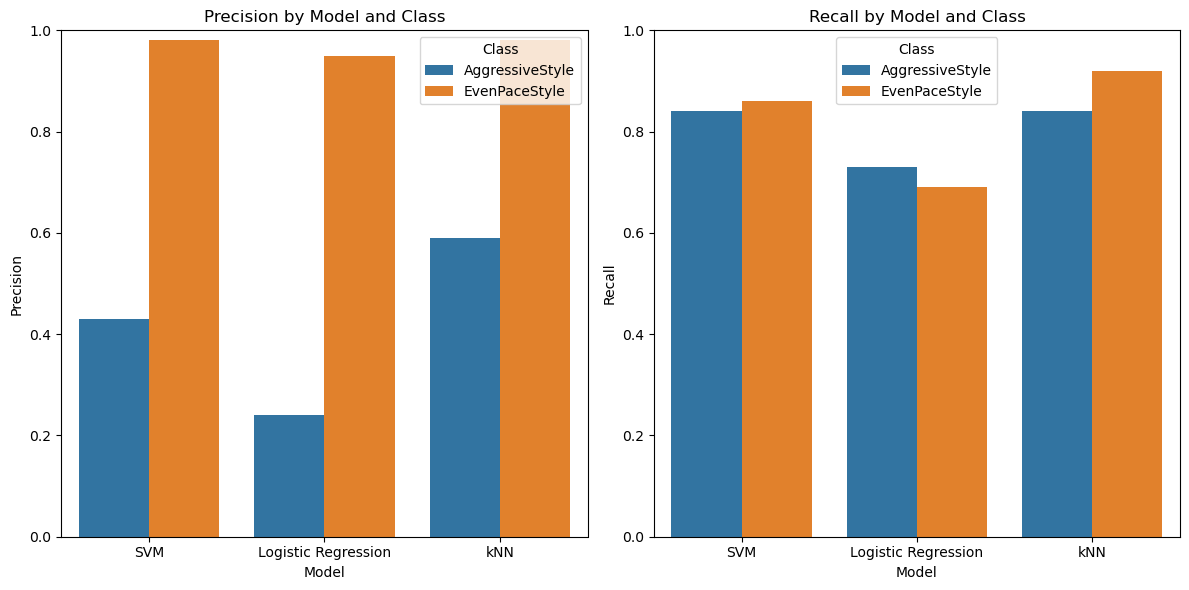
\includegraphics[width=0.5\textwidth]{images/comparison1.png}
    \caption{Precision and Recall comparison}
    \label{fig:enter-label}
\end{figure}

\begin{figure}[h]
    \centering
    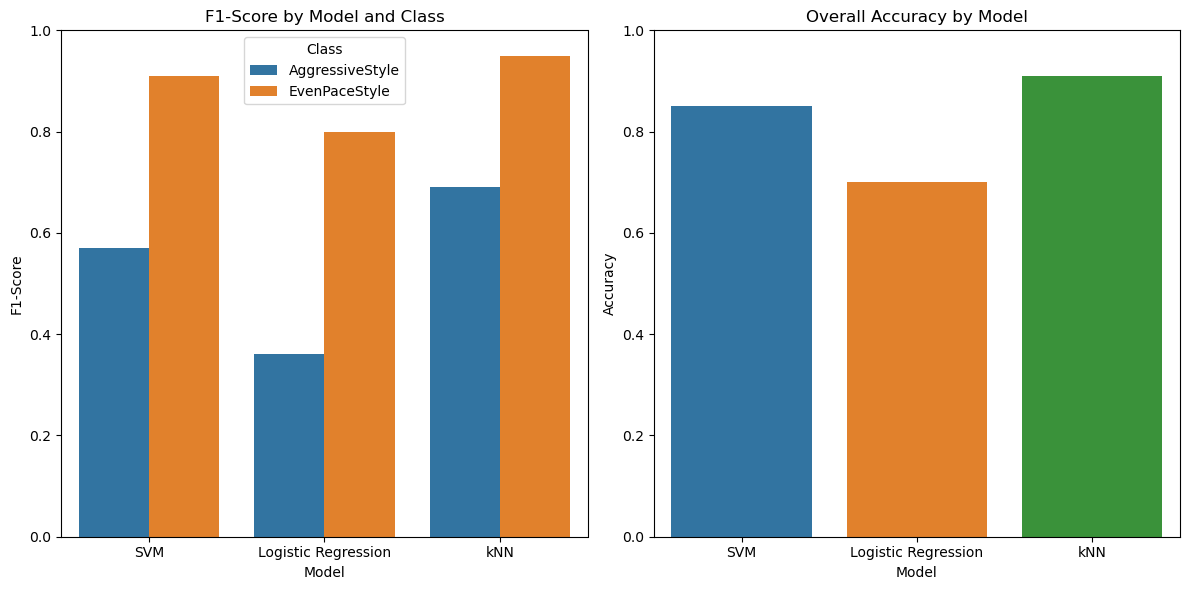
\includegraphics[width=0.5\textwidth]{images/comparison2.png}
    \caption{F1-Score and Accuracy comparison}
    \label{fig:enter-label}
\end{figure}

\section{Conclusion}
By comparing Logistic Regression, Support Vector Machine (SVM) and K-Nearest Neighbors (KNN) algorithms, the analysis revealed that kNN displayed a superior accuracy and balanced metrics, proving most effective to this application. SVM shoed an impressive recall, particularly for identifying the \textbf{AggressiveStyle} driving, with Logistic Regression offering interpretability, although with lower precision, showcasing the strengths of each algorithm.
In conclusion, the project highlights the importance of rigorous data preprocessing and cross-validation. While the performance may vary across different attributes, it can be concluded that the classifiers generally perform well for the driving style prediction, with F1-Scores above \textit{0.8} in the most effective classifier. One observation is that models prioritising interpretability tend to perform poorly, highlighting the trade-off between interpretability and accuracy.


% references section
\printbibliography

\end{document}